\documentclass[10pt]{article}

\usepackage{float}
\usepackage{cite}
\usepackage{amsmath}
\usepackage{mathtools}
\usepackage{booktabs}
\usepackage{graphicx}
\usepackage{epstopdf}
\usepackage{multicol}
\usepackage{geometry}

\newcommand{\sens}{\mbox{ sens }}
\newcommand{\spec}{\mbox{ spec }}

\newcommand{\mgin}{0.5in}
\geometry{
    left=\mgin,
    right=\mgin,
    top=\mgin,
    bottom=\mgin
}

% Font
\usepackage{calligra}
\usepackage{libertine}
\usepackage{tgpagella}
\usepackage[T1]{fontenc}


%%fakesection title
\begin{document}
\null

\thispagestyle{empty}
\addtocounter{page}{-1}

\begin{center}
  \begin{sffamily}
	\begin{bfseries}
	  \null
	  \vfill
	  \Huge{Machine Learning with Python to Diagnose Chiari Malformation Type I} \\
	  \vspace{20pt}
	\end{bfseries}
  \end{sffamily}
  \begin{Large}
	Oliver Evans \\
	Dr. Malena Espa\~nol \\
	University of Akron \\
	\vspace{20pt}
	\today
  \end{Large}
  \vspace{30pt}

  \null
  \vfill
  \vfill
  \null
\end{center}
\pagebreak

\section{Introduction}
We have built on the work done by Urbizu et al. \cite{urbizu} in investigating the potential for machine learning in assisting in the diagnosis of Chiari Malformation Type I (CMI). MRI data has been shown to be very useful in diagnosing CMI. Currently, Tonsillar Descent is the primary feature used in diagnosis, although it does not always correctly characterize CMI. We seek to find a correlation between other MRI measurements and CMI diagnosis. \\

We have used Python and the machine learning algorithms included in the scikit-learn\cite{scikit-learn} package. We used the following algorithms in our investigation: Support Vector Machines (SVM), 4 Nearest Neighbors (4NN), Decision Tree (DT), Linear Discriminant Analysis (LDA), Naive-Bayesian (NB), Linear Regression (LR)

\section{Data}
We have MRI measurements from 100 CMI patients and 50 controls (non-CMI) for the following features from Urbizu et al. We also have data about symptoms for each of the CMI patients. \\

\begin{figure}[H]
	\noindent
	\begin{tabular}{ll}
		\toprule
		Feature \# & Feature Name \\
		\midrule
		0 & TD \\
		1 & Tentorium \\
		2 & Supraoccipital \\
		3 & FM \\
		4 & Clivus \\
		5 & FCP area \\
		6 & Osseus FCP area \\
		7 & Corpus Callosum to FM \\
		8 & Height PCF \\
		9 & Width PCF \\
		10 & Fastigium to FM \\
		11 & Pons to FM \\
		12 & Basal angulation \\
		13 & Tentorium angle \\
		14 & Wackenheim angle \\
		15 & Basilar impression \\
		16 & Odontoid angle \\
		\bottomrule
	\end{tabular}
	\hspace{5em}
	\begin{tabular}{ll}
		\toprule
		Symptom Name & Symptom Name \\
		\midrule
		Asymptomatic &  Fatigue \\ 
		Occipital neck headace &        Instability \\ 
		Bifrontal headace &     Sensory Loss \\ 
		Holocranial headace &   Anxiety \\ 
		Hemicranial headace &   Depression \\ 
		Any Headache &  Motor Weakness \\ 
		Hydrocephalus &         Dysphagia \\ 
		Syringomyelia &         Dysphonia \\ 
		Pseudotumor Cerebri &   Gait Disturbances \\ 
		Complex Craniocervical Malformation &   Paresthesia Upper Limbs \\ 
		Klippel-Feil Malformation &     Paresthesia Lower Limbs \\ 
		Retrocurved Odontoid &  Upper Limbs Pain \\ 
		Other CVJ Malformations &       Lower Limbs Pain \\ 
		Cough Headaches &       Neck Pain \\ 
		Dizziness &     Difficulty Swallowing \\ 
		Vertigo &       Nystagmus \\ 
		Visual Alterations &    Kyphoscoliosis \\
		\bottomrule
	\end{tabular}
	\caption{List of Features and Symptoms}
\end{figure}

\section{Method}
Our primary goal was to effectively distinguish CMI patients from controls based on other MRI symptoms. To do this, we took all possible unordered combinations of 2-7 features and applied all of the above-listed algorithms in order to classify all samples as CMI or non-CMI, where a sample is either a CMI patient or a control. Let each of these combinations of features be called a tuple and each application of an algorithm to a tuple be called a trial. In each trial, the samples were divided into five sets each containing similar proportions of CMI and non-CMI samples. We used each set as a training dataset while the union of the other sets was used for testing. We calculated the average sensitivity and specificity obtained by using each of the five training sets, and reported these as the sensitivity and specificity for the trial. Then, for each algorithm, for each tuple size, we selected the tuple of that size which most successfully distinguished between CMI and non-CMI samples. In the following pages, we report the sensitivity, specificity, and tuple which we deemed most successful for each tuple size and algorithm.

Our next step was to attempt to isolate our CMI patients (ignore controls) and attempt to predict whether or not each patient experienced each of the above-listed symptoms. We performed a slightly simplified version of the previous procedure for each symptom, where we chose only the single combination of tuple and algorithm which most effectively distinguished between CMI patients and controls.

\pagebreak
\section{Defining Effective Classification}
In seeking to choose the best among a set of trials, it becomes necessary to define a metric for comparison. For each trial, we know primarily the sensitivity and specificity, and so we will use these as the building blocks of our metrics. We use four metrics for comparing trials, each of which is a simple function of sensitivity and specificity. We call them ``sum'', ``prod'' for product, ``perf`` for performance, and ''alpha`` for lack of a better term. Each of these metrics aims to favor trials with higher sensitivity and specificity. We should begin by defining the sensitivity and specificity of a trial. Let the events $C$ and $NC$ represent an individual having CMI and not having CMI respectively. Let the events $TP$ (''test positive``) and $TN$(''test negative``) represent an individual being classified by the algorithm (perhaps incorrectly) as CMI and non-CMI respectively. We denote the sensitivity by ``sens'' and the specificity by ``spec''. \\

Then for a given trial,
\begin{align}
	\sens &= P(TP|C) \\
	\spec &= P(TN|NC)
\end{align}

We should also state two other useful probability relationships. \\

Firstly, Bayes' Theorem:
\begin{equation}
	P(A|B)P(B) = P(B|A)P(A) = P(A) \cap P(B)
\end{equation}

Secondly, if $P(A) + P(B) = 1$, then
\begin{equation}
	P(C|A)P(A) + P(C|B)P(B) = P(C)
\end{equation}

Note that $P(TP) + P(TN) = 1$ and $P(C) + P(NC) = 1$. \\

\subsection{sum}
Our first metric is a simple sum. It fails to sufficiently penalize zero-values of sensitivity or specificity, which, in some cases results in inappropriately choosing a trial which has entirely failed, classifying the all of the samples as either CMI or non-CMI, yielding a sensitivity of 1 and specificity of 0 or vice versa.
\begin{equation}
	\mbox{sum } = \sens + \spec
\end{equation}

\subsection{prod}
Taking the product of the sensitivity and specificity successfully penalizes zero or almost-zero values for sensitivity or specificity, avoiding total failures which were problematic in the previous case.
\begin{equation}
	\mbox{prod } = \sens\cdot\spec
\end{equation}

\subsection{perf}
Another straightforward metric is simply the percentage of samples which were correctly classified, regardless of whether they are CMI patients or controls.
This can be represented as 
\begin{align*}
	\mbox{perf } &= P(TP \cap C) + P(TN \cap NC) \\
	&= P(TP|C)\tilde{P}(C) + P(TN|NC)\tilde{P}(NC)
\end{align*}

where $\tilde{P}$ represents the occurrence within our data set, not within the general population. Then since we have 100 CMI patients and 50 controls, $\tilde{P}(C) = \frac{2}{3}$ and $\tilde{P}(NC) = \frac{1}{3}$. Therefore, 
\begin{equation}
	\mbox{perf } = \frac{2}{3}\sens + \frac{1}{3}\spec
\end{equation}

\subsection{alpha}
Sensitivity and specificity are useful classifiers of a statistical test, but they are not so useful for a patient receiving a diagnosis. A patient is not interested in the probability that they will be correctly classified \emph{if} they have the disease. Rather they are concerned with the probability that if they are classified, they \emph{do} have the disease. Therefore, we would like to use the quantity $P(C|TP)$ as a metric. We call this quantity alpha ($\tilde\alpha$).

\begin{align*}
	\tilde\alpha &= P(C|TP) \\[1em]
		&= \frac{P(TP|C)P(C)}{P(TP)} \\[1em]
		&= \frac{P(TP|C)P(C)}{P(TP|C)P(C) + P(TP|NC)P(NC)} \\[1em]
		&= \frac{P(TP|C)P(C)}{P(TP|C)P(C) + P(TP|NC)(1-P(C))} \\[1em]
		&= \frac{P(TP|C)P(C)}{P(TP|NC) + P(C)[P(TP|C) - P(TP|NC)]} \\[1em]
		&= \frac{P(TP|C)}{\frac{1}{P(C)}P(TP|NC) + P(TP|C) - P(TP|NC)} \\[1em]
		&= \frac{P(TP|C)}{P(TP|NC)(\frac{1}{P(C)}-1) + P(TP|C)} \\[1em]
		&= \frac{1}{\frac{P(TP|NC)}{P(TP|C)}(\frac{1}{P(C)}-1) + 1} \\[1em]
		&= \frac{1}{\frac{1-P(TN|NC)}{P(TP|C)}(\frac{1}{P(C)}-1) + 1} \\[1em]
		&= \left[\frac{1-\spec}{\sens}\left(\frac{1}{P(C)} - 1 \right) + 1 \right]^{-1} \\[1em]
\end{align*}

Notice that we now have $P(C)$ in our equation, which is the prevalence of CMI among the whole population. We assume that this is unknown. Luckily, we can define a new quantity, $\alpha$, and show that using $\alpha$ as a metric for comparison is equivalent to using $\tilde\alpha$. \\

Let
\begin{equation}
	\alpha = \frac{\sens}{1-\spec}.
\end{equation}

Assume we have two trials, A and B which we seek to compare. Let $x_A$ and $y_A$ be sens and spec values for trial A respectively, and let $x_B$ and $y_B$ be the corresponding values for trial B. Assume it has been shown that by comparing $\tilde\alpha$ values, trial B has been deemed more effective. That is,

\begin{align*}
	\tilde\alpha_A &< \tilde\alpha_B \\[1em]
&\Leftrightarrow \\[1em]
	\left[\frac{1-y_A}{x_A}\left(\frac{1}{P(C)} - 1 \right) + 1 \right]^{-1} &< 
	\left[\frac{1-y_B}{x_B}\left(\frac{1}{P(C)} - 1 \right) + 1 \right]^{-1} \\[1em]
&\Leftrightarrow \\[1em]
	\frac{1-y_B}{x_B}\left(\frac{1}{P(C)} - 1 \right) + 1  &<
	\frac{1-y_A}{x_A}\left(\frac{1}{P(C)} - 1 \right) + 1  \\[1em] 
&\Leftrightarrow \\[1em]
	\frac{1-y_B}{x_B} &<
	\frac{1-y_A}{x_A} \\[1em] 
&\Leftrightarrow \\[1em]
	\frac{x_A}{1-y_A} &<
	\frac{x_B}{1-y_B} \\[1em]
&\Leftrightarrow \\[1em]
	\alpha_A &< \alpha_B
\end{align*}

Since all of the above operations hold in both directions (assuming $0 < P(C),\sens,\spec < 1$), $\alpha$ and $\tilde\alpha$ are equivalent metrics.

\section{Results}
In the following pages, we present the tables discussed previously: The sensitivity, specificity and feature numbers of the tuple for which each algorithm is most effective for each tuple size. These results are given for all of the previously discussed metrics. Also shown is a contour map of each metric as a function of sensitivity and specificity. A trial which receives a sensitivity and specificity rating pair which falls, for example, on a red contour line in the contour map will be judged by that metric as superior to a trial which results in a rating pair on a blue contour line. \\

On the final page of results is the outcome of our attempt to predict individual symptoms from MRI measurements. The single best trial according to the ``prod'' metric is shown in the table in all cases where classification was successful, along with the prod, sens, spec, and perf values for that trial. In some symptoms for which there was not enough data to successfully attempt classification, a blank line is shown. Above the table is a bar chart comparing the four previously-mentioned quantities for each symptom with at least one successful trial.

\pagebreak
\subsection{sum}
\vspace{1em}
\begin{equation}
	\mbox{sum } = \sens + \spec
\end{equation}
\vspace{1em}

\begin{multicols}{2}
	\begin{figure}[H]
		\center
		\input{../tables/sum/sens.tex}
		\caption{Sensitivity (sum)}
	\end{figure}

	\begin{figure}[H]
		\center
		\input{../tables/sum/spec.tex}
		\caption{Specificity (sum)}
	\end{figure}
	
	\begin{figure}[H]
		\includegraphics{../tables/sum/contour}
	\end{figure}
\end{multicols}

\vspace{2em}

\begin{figure}[H]
	\center
	\input{../tables/sum/tuples.tex}
	\caption{Best Tuples (sum)}
\end{figure}

\pagebreak
\subsection{prod}
\vspace{1em}
\begin{equation}
	\mbox{prod } = \sens\cdot\spec
\end{equation}
\vspace{1em}

\begin{multicols}{2}
	\begin{figure}[H]
		\center
		\input{../tables/prod/sens.tex}
		\caption{Sensitivity (prod)}
	\end{figure}

	\begin{figure}[H]
		\center
		\input{../tables/prod/spec.tex}
		\caption{Specificity (prod)}
	\end{figure}
	
	\begin{figure}[H]
		\includegraphics{../tables/prod/contour}
	\end{figure}
\end{multicols}

\vspace{2em}

\begin{figure}[H]
	\center
	\input{../tables/prod/tuples.tex}
	\caption{Best Tuples (prod)}
\end{figure}

\pagebreak
\subsection{perf}
\vspace{1em}
\begin{equation}
	\mbox{perf } = \frac{2}{3}\sens + \frac{1}{3}\spec
\end{equation}
\vspace{1em}

\begin{multicols}{2}
	\begin{figure}[H]
		\center
		\input{../tables/perf/sens.tex}
		\caption{Sensitivity (perf)}
	\end{figure}

	\begin{figure}[H]
		\center
		\input{../tables/perf/spec.tex}
		\caption{Specificity (perf)}
	\end{figure}
	
	\begin{figure}[H]
		\includegraphics{../tables/perf/contour}
	\end{figure}
\end{multicols}

\vspace{2em}

\begin{figure}[H]
	\center
	\input{../tables/perf/tuples.tex}
	\caption{Best Tuples (perf)}
\end{figure}

\pagebreak
\subsection{alpha}
\vspace{1em}
\begin{equation}
	\alpha = \frac{\sens}{1-\spec}
\end{equation}
\vspace{1em}

\begin{multicols}{2}
	\begin{figure}[H]
		\center
		\input{../tables/alpha/sens.tex}
		\caption{Sensitivity (alpha)}
	\end{figure}

	\begin{figure}[H]
		\center
		\input{../tables/alpha/spec.tex}
		\caption{Specificity (alpha)}
	\end{figure}
	
	\begin{figure}[H]
		\includegraphics{../tables/alpha/contour}
	\end{figure}
\end{multicols}

\vspace{2em}

\begin{figure}[H]
	\center
	\input{../tables/alpha/tuples.tex}
	\caption{Best Tuples (alpha)}
\end{figure}




\begin{figure}[H]
    \centering
    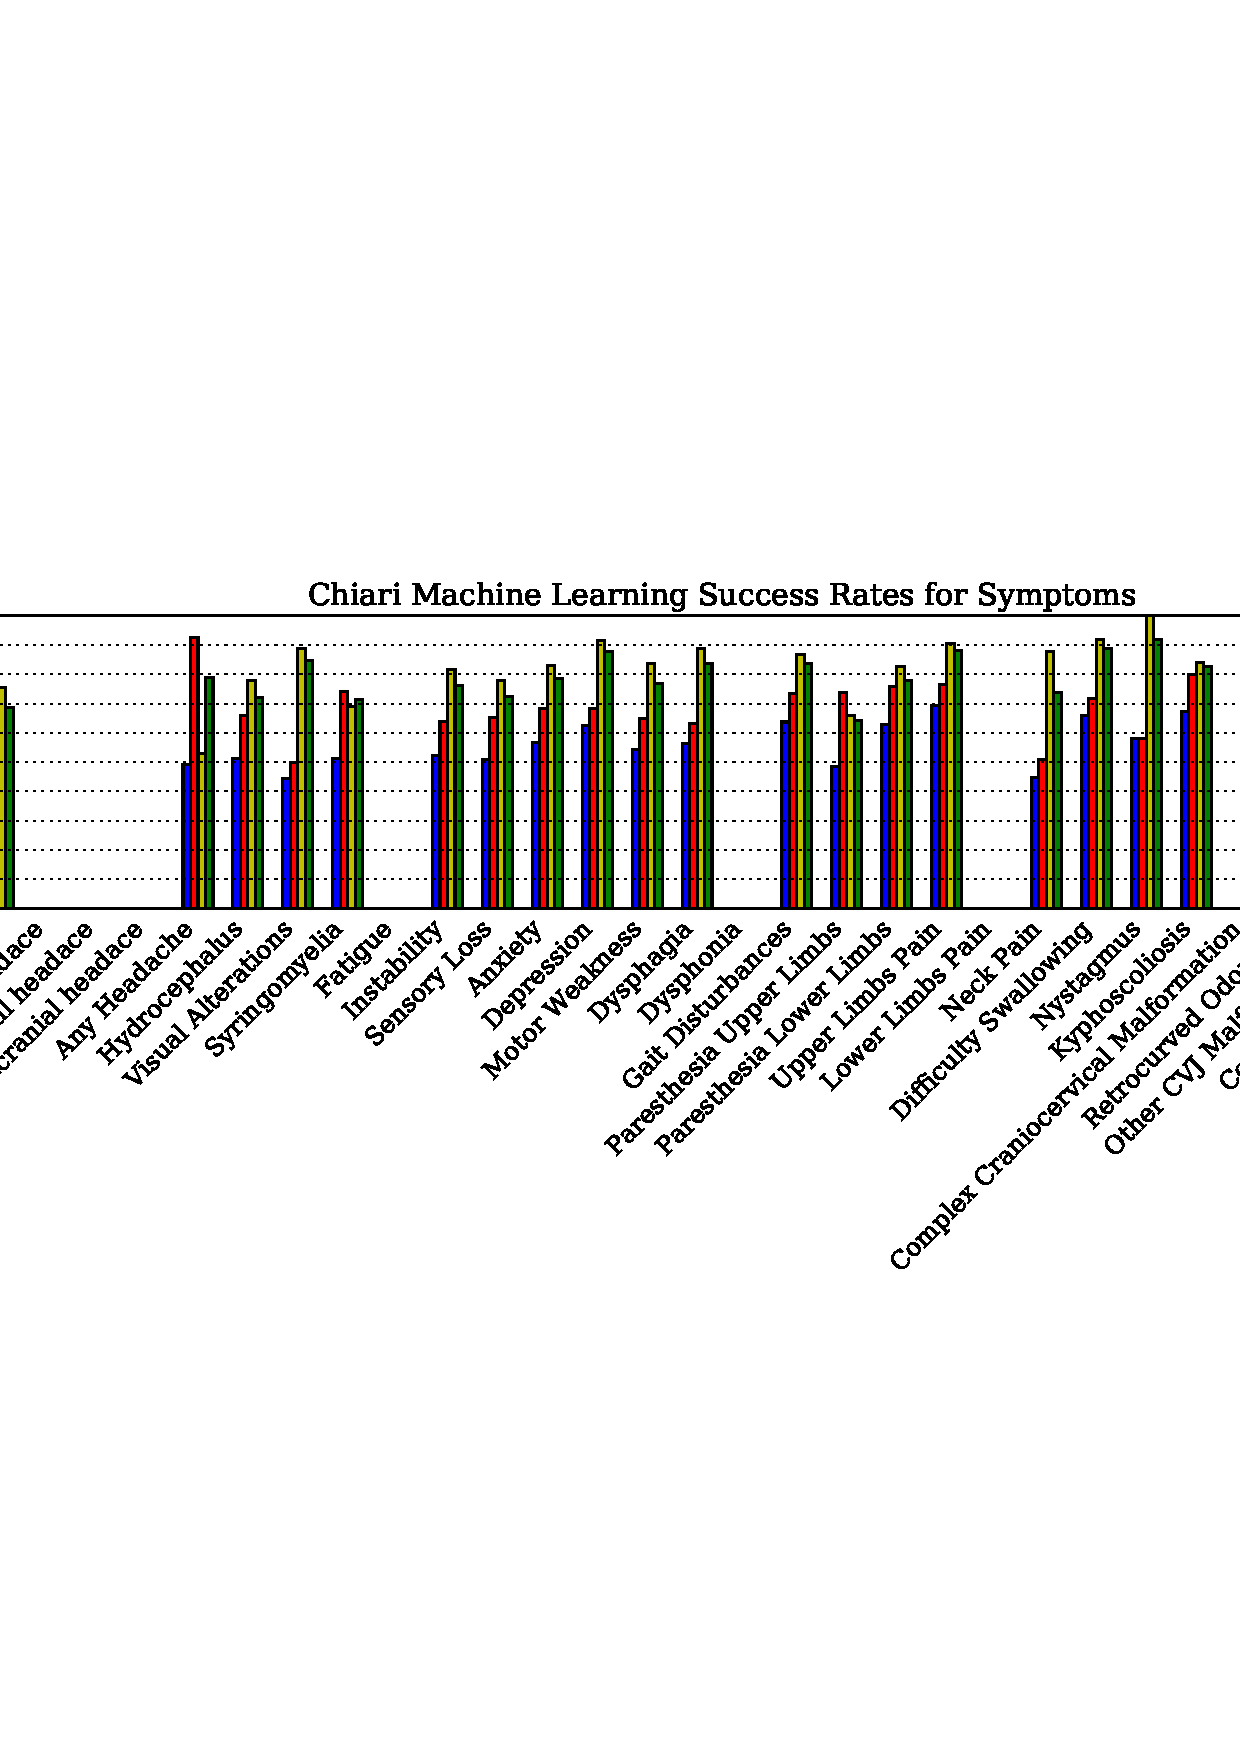
\includegraphics[width=\textwidth]{symptom_success_plot.pdf}
    \begin{tabular}{lllllll}
\toprule
                             Symptom &                 Best Tuple & Algorithm & prod & sens & spec & perf \\
\midrule
                        Asymptomatic &                            &           &      &      &      &      \\
              Occipital neck headace &            (8, 10, 11, 15) &        DT & 0.47 & 0.62 & 0.76 & 0.69 \\
                   Bifrontal headace &                            &           &      &      &      &      \\
                 Holocranial headace &                            &           &      &      &      &      \\
                 Hemicranial headace &                            &           &      &      &      &      \\
                        Any Headache &         (4, 6, 13, 15, 16) &       LDA & 0.49 & 0.93 & 0.53 & 0.79 \\
                       Hydrocephalus &  (6, 7, 8, 10, 11, 12, 13) &        DT & 0.51 & 0.66 & 0.78 & 0.72 \\
                  Visual Alterations &  (3, 5, 8, 11, 12, 13, 14) &        DT & 0.44 & 0.50 & 0.89 & 0.85 \\
                       Syringomyelia &                    (2, 12) &        DT & 0.51 & 0.74 & 0.69 & 0.72 \\
                             Fatigue &                            &           &      &      &      &      \\
                         Instability &               (12, 14, 15) &        DT & 0.52 & 0.64 & 0.82 & 0.76 \\
                        Sensory Loss &  (4, 7, 9, 11, 12, 13, 15) &        DT & 0.51 & 0.65 & 0.78 & 0.72 \\
                             Anxiety &              (2, 5, 9, 12) &        DT & 0.57 & 0.68 & 0.83 & 0.79 \\
                          Depression &    (2, 5, 6, 8, 9, 15, 16) &        DT & 0.62 & 0.68 & 0.91 & 0.88 \\
                      Motor Weakness &           (4, 6, 7, 8, 11) &        DT & 0.54 & 0.65 & 0.84 & 0.77 \\
                           Dysphagia &          (4, 5, 6, 10, 11) &        DT & 0.56 & 0.63 & 0.89 & 0.84 \\
                           Dysphonia &                            &           &      &      &      &      \\
                   Gait Disturbances &         (4, 5, 10, 13, 15) &        DT & 0.64 & 0.73 & 0.87 & 0.84 \\
             Paresthesia Upper Limbs &     (2, 8, 10, 13, 15, 16) &        DT & 0.49 & 0.74 & 0.66 & 0.64 \\
             Paresthesia Lower Limbs &      (3, 7, 9, 13, 14, 16) &        DT & 0.63 & 0.76 & 0.83 & 0.78 \\
                    Upper Limbs Pain &      (4, 7, 8, 11, 12, 13) &        DT & 0.69 & 0.77 & 0.91 & 0.88 \\
                    Lower Limbs Pain &                            &           &      &      &      &      \\
                           Neck Pain &      (2, 3, 6, 12, 13, 14) &       QDA & 0.45 & 0.51 & 0.88 & 0.74 \\
               Difficulty Swallowing &             (4, 8, 11, 16) &        DT & 0.66 & 0.72 & 0.92 & 0.89 \\
                           Nystagmus &          (2, 4, 6, 10, 11) &       QDA & 0.58 & 0.58 & 1.00 & 0.92 \\
                      Kyphoscoliosis &     (6, 9, 11, 12, 13, 14) &        DT & 0.67 & 0.80 & 0.84 & 0.83 \\
 Complex Craniocervical Malformation &                            &           &      &      &      &      \\
                Retrocurved Odontoid &      (2, 3, 4, 11, 12, 15) &        DT & 0.63 & 0.68 & 0.92 & 0.87 \\
             Other CVJ Malformations &             (4, 6, 14, 16) &        DT & 0.56 & 0.67 & 0.85 & 0.82 \\
                     Cough Headaches &   (2, 5, 8, 9, 10, 12, 15) &       QDA & 0.52 & 0.73 & 0.71 & 0.71 \\
                           Dizziness &             (4, 6, 12, 14) &        DT & 0.49 & 0.62 & 0.80 & 0.74 \\
                             Vertigo &                            &           &      &      &      &      \\
\bottomrule
\end{tabular}

	\caption{Classification results for symptoms based on the product of sensitivity and specificity}
\end{figure}

\pagebreak
\bibliographystyle{plain}
\bibliography{references}

\end{document}
